% Options for packages loaded elsewhere
\PassOptionsToPackage{unicode}{hyperref}
\PassOptionsToPackage{hyphens}{url}
%
\documentclass[
  man]{apa6}
\usepackage{amsmath,amssymb}
\usepackage{iftex}
\ifPDFTeX
  \usepackage[T1]{fontenc}
  \usepackage[utf8]{inputenc}
  \usepackage{textcomp} % provide euro and other symbols
\else % if luatex or xetex
  \usepackage{unicode-math} % this also loads fontspec
  \defaultfontfeatures{Scale=MatchLowercase}
  \defaultfontfeatures[\rmfamily]{Ligatures=TeX,Scale=1}
\fi
\usepackage{lmodern}
\ifPDFTeX\else
  % xetex/luatex font selection
\fi
% Use upquote if available, for straight quotes in verbatim environments
\IfFileExists{upquote.sty}{\usepackage{upquote}}{}
\IfFileExists{microtype.sty}{% use microtype if available
  \usepackage[]{microtype}
  \UseMicrotypeSet[protrusion]{basicmath} % disable protrusion for tt fonts
}{}
\makeatletter
\@ifundefined{KOMAClassName}{% if non-KOMA class
  \IfFileExists{parskip.sty}{%
    \usepackage{parskip}
  }{% else
    \setlength{\parindent}{0pt}
    \setlength{\parskip}{6pt plus 2pt minus 1pt}}
}{% if KOMA class
  \KOMAoptions{parskip=half}}
\makeatother
\usepackage{xcolor}
\usepackage{graphicx}
\makeatletter
\def\maxwidth{\ifdim\Gin@nat@width>\linewidth\linewidth\else\Gin@nat@width\fi}
\def\maxheight{\ifdim\Gin@nat@height>\textheight\textheight\else\Gin@nat@height\fi}
\makeatother
% Scale images if necessary, so that they will not overflow the page
% margins by default, and it is still possible to overwrite the defaults
% using explicit options in \includegraphics[width, height, ...]{}
\setkeys{Gin}{width=\maxwidth,height=\maxheight,keepaspectratio}
% Set default figure placement to htbp
\makeatletter
\def\fps@figure{htbp}
\makeatother
\setlength{\emergencystretch}{3em} % prevent overfull lines
\providecommand{\tightlist}{%
  \setlength{\itemsep}{0pt}\setlength{\parskip}{0pt}}
\setcounter{secnumdepth}{-\maxdimen} % remove section numbering
% Make \paragraph and \subparagraph free-standing
\ifx\paragraph\undefined\else
  \let\oldparagraph\paragraph
  \renewcommand{\paragraph}[1]{\oldparagraph{#1}\mbox{}}
\fi
\ifx\subparagraph\undefined\else
  \let\oldsubparagraph\subparagraph
  \renewcommand{\subparagraph}[1]{\oldsubparagraph{#1}\mbox{}}
\fi
\newlength{\cslhangindent}
\setlength{\cslhangindent}{1.5em}
\newlength{\csllabelwidth}
\setlength{\csllabelwidth}{3em}
\newlength{\cslentryspacingunit} % times entry-spacing
\setlength{\cslentryspacingunit}{\parskip}
\newenvironment{CSLReferences}[2] % #1 hanging-ident, #2 entry spacing
 {% don't indent paragraphs
  \setlength{\parindent}{0pt}
  % turn on hanging indent if param 1 is 1
  \ifodd #1
  \let\oldpar\par
  \def\par{\hangindent=\cslhangindent\oldpar}
  \fi
  % set entry spacing
  \setlength{\parskip}{#2\cslentryspacingunit}
 }%
 {}
\usepackage{calc}
\newcommand{\CSLBlock}[1]{#1\hfill\break}
\newcommand{\CSLLeftMargin}[1]{\parbox[t]{\csllabelwidth}{#1}}
\newcommand{\CSLRightInline}[1]{\parbox[t]{\linewidth - \csllabelwidth}{#1}\break}
\newcommand{\CSLIndent}[1]{\hspace{\cslhangindent}#1}
\ifLuaTeX
\usepackage[bidi=basic]{babel}
\else
\usepackage[bidi=default]{babel}
\fi
\babelprovide[main,import]{english}
% get rid of language-specific shorthands (see #6817):
\let\LanguageShortHands\languageshorthands
\def\languageshorthands#1{}
% Manuscript styling
\usepackage{upgreek}
\captionsetup{font=singlespacing,justification=justified}

% Table formatting
\usepackage{longtable}
\usepackage{lscape}
% \usepackage[counterclockwise]{rotating}   % Landscape page setup for large tables
\usepackage{multirow}		% Table styling
\usepackage{tabularx}		% Control Column width
\usepackage[flushleft]{threeparttable}	% Allows for three part tables with a specified notes section
\usepackage{threeparttablex}            % Lets threeparttable work with longtable

% Create new environments so endfloat can handle them
% \newenvironment{ltable}
%   {\begin{landscape}\centering\begin{threeparttable}}
%   {\end{threeparttable}\end{landscape}}
\newenvironment{lltable}{\begin{landscape}\centering\begin{ThreePartTable}}{\end{ThreePartTable}\end{landscape}}

% Enables adjusting longtable caption width to table width
% Solution found at http://golatex.de/longtable-mit-caption-so-breit-wie-die-tabelle-t15767.html
\makeatletter
\newcommand\LastLTentrywidth{1em}
\newlength\longtablewidth
\setlength{\longtablewidth}{1in}
\newcommand{\getlongtablewidth}{\begingroup \ifcsname LT@\roman{LT@tables}\endcsname \global\longtablewidth=0pt \renewcommand{\LT@entry}[2]{\global\advance\longtablewidth by ##2\relax\gdef\LastLTentrywidth{##2}}\@nameuse{LT@\roman{LT@tables}} \fi \endgroup}

% \setlength{\parindent}{0.5in}
% \setlength{\parskip}{0pt plus 0pt minus 0pt}

% Overwrite redefinition of paragraph and subparagraph by the default LaTeX template
% See https://github.com/crsh/papaja/issues/292
\makeatletter
\renewcommand{\paragraph}{\@startsection{paragraph}{4}{\parindent}%
  {0\baselineskip \@plus 0.2ex \@minus 0.2ex}%
  {-1em}%
  {\normalfont\normalsize\bfseries\itshape\typesectitle}}

\renewcommand{\subparagraph}[1]{\@startsection{subparagraph}{5}{1em}%
  {0\baselineskip \@plus 0.2ex \@minus 0.2ex}%
  {-\z@\relax}%
  {\normalfont\normalsize\itshape\hspace{\parindent}{#1}\textit{\addperi}}{\relax}}
\makeatother

\makeatletter
\usepackage{etoolbox}
\patchcmd{\maketitle}
  {\section{\normalfont\normalsize\abstractname}}
  {\section*{\normalfont\normalsize\abstractname}}
  {}{\typeout{Failed to patch abstract.}}
\patchcmd{\maketitle}
  {\section{\protect\normalfont{\@title}}}
  {\section*{\protect\normalfont{\@title}}}
  {}{\typeout{Failed to patch title.}}
\makeatother

\usepackage{xpatch}
\makeatletter
\xapptocmd\appendix
  {\xapptocmd\section
    {\addcontentsline{toc}{section}{\appendixname\ifoneappendix\else~\theappendix\fi\\: #1}}
    {}{\InnerPatchFailed}%
  }
{}{\PatchFailed}
\keywords{keywords\newline\indent Word count: X}
\DeclareDelayedFloatFlavor{ThreePartTable}{table}
\DeclareDelayedFloatFlavor{lltable}{table}
\DeclareDelayedFloatFlavor*{longtable}{table}
\makeatletter
\renewcommand{\efloat@iwrite}[1]{\immediate\expandafter\protected@write\csname efloat@post#1\endcsname{}}
\makeatother
\usepackage{lineno}

\linenumbers
\usepackage{csquotes}
\ifLuaTeX
  \usepackage{selnolig}  % disable illegal ligatures
\fi
\IfFileExists{bookmark.sty}{\usepackage{bookmark}}{\usepackage{hyperref}}
\IfFileExists{xurl.sty}{\usepackage{xurl}}{} % add URL line breaks if available
\urlstyle{same}
\hypersetup{
  pdftitle={Can we really harvest insights for rice theory from two state farms in China?},
  pdfauthor={Anjie Cao1},
  pdflang={en-EN},
  pdfkeywords={keywords},
  hidelinks,
  pdfcreator={LaTeX via pandoc}}

\title{Can we really harvest insights for rice theory from two state farms in China?}
\author{Anjie Cao\textsuperscript{1}}
\date{}


\shorttitle{Rice theory comment}

\authornote{

Add complete departmental affiliations for each author here. Each new line herein must be indented, like this line.

Enter author note here.

Correspondence concerning this article should be addressed to Anjie Cao, 450 Jane Stanford Way, Stanford, CA 94305. E-mail: \href{mailto:anjiecao@stanford.edu}{\nolinkurl{anjiecao@stanford.edu}}

}

\affiliation{\vspace{0.5cm}\textsuperscript{1} Stanford University}

\abstract{%
Mid-20th century in the People's Republic of China was a turbulent period: wars, famines, and Cultural Revolution that disrupted lives for a decade and more. Under this historical context, two state farms, Lianhu and Qukou were founded and developed. According to Talheim \& Dong (2024), Lianhu is a rice farm and Qukou is a wheat farm. Since the farmers in the two farms were mostly randomly assigned to work on these farms, this pair of farms created a rare natural experiment to test the causal relationship between farming practices and their cultural orientation: i.e.~farming rice leads people to become more collectivistic (Talhelm et al., 2014). But do these two farms really provide a clear causal test for the effect of farming practices? In this comment, I show that the strengths of the three experimental effects in the paper have different degrees of sensitivity towards analytical decisions, which creates challenges in interpreting the empirical evidence. Furthermore, I argue that the historical context of the two farms may have played an important role in shaping the cultural orientation. The differences observed across two farms could be attributed to factors other than farming practices.
}



\begin{document}
\maketitle

Mid-20th century in the People's Republic of China was a turbulent period: wars, famines, and Cultural Revolution that disrupted lives for a decade and more. Under this historical context, two state farms, Lianhu and Qukou were founded and developed. According to Talhelm and Dong (2024), Lianhu is a rice farm and Qukou is a wheat farm. Since the farmers in the two farms were mostly randomly assigned to work on these farms, this pair of farms created a rare natural experiment to test the causal relationship between farming practices and their cultural orientation: i.e.~farming rice leads people to become more collectivistic (Talhelm et al., 2014). But do these two farms really provide a clear causal test for the effect of farming practices? In this comment, I show that the strengths of the three experimental effects in the paper have different degrees of sensitivity towards analytical decisions, which creates challenges in interpreting the empirical evidence. Furthermore, I argue that the historical context of the two farms may have played an important role in shaping the cultural orientation. The differences observed across two farms could be attributed to factors other than farming practices.

To isolate the effect of farming practice, the main analyses in Talhelm and Dong (2024) used both controlling for variables in regression and propensity score matching. Five demographic variables were chosen: age, gender, maternal education, family income, and ethnicity (whether someone self-identified as Hui or not). All variables but the ethnicity were used in the propensity score matching procedure. Since this analysis was not preregistered and the variables were post-hoc selected from all demographic information collected, it is critical to examine the robustness of the effect to different model specifications. I ran a multiverse analysis by including all possible subsets of the five variables on either matched and unmatched datasets for the three main tasks: Self-Inflation (Family), Loyalty/Nepotism, and the Relational Categorization task. All three tasks were assumed to be implicit measures of individualism (Figure 1). However, the analysis showed that only the Self-inflation (Family) was robust to different analytic strategies. In contrast, Loyalty/Nepotism task was particularly sensitive to the propensity score matching procedure, and the Relational Categorization task was sensitive to the model specifications. This heterogeneous pattern highlights the importance of taking into account analytical flexibility in interpreting results, and invites one to consider to what extent these variations might reflect underlying methodological challenges or actual differences in psychological constructs across the two farms.

\begin{figure}
\centering
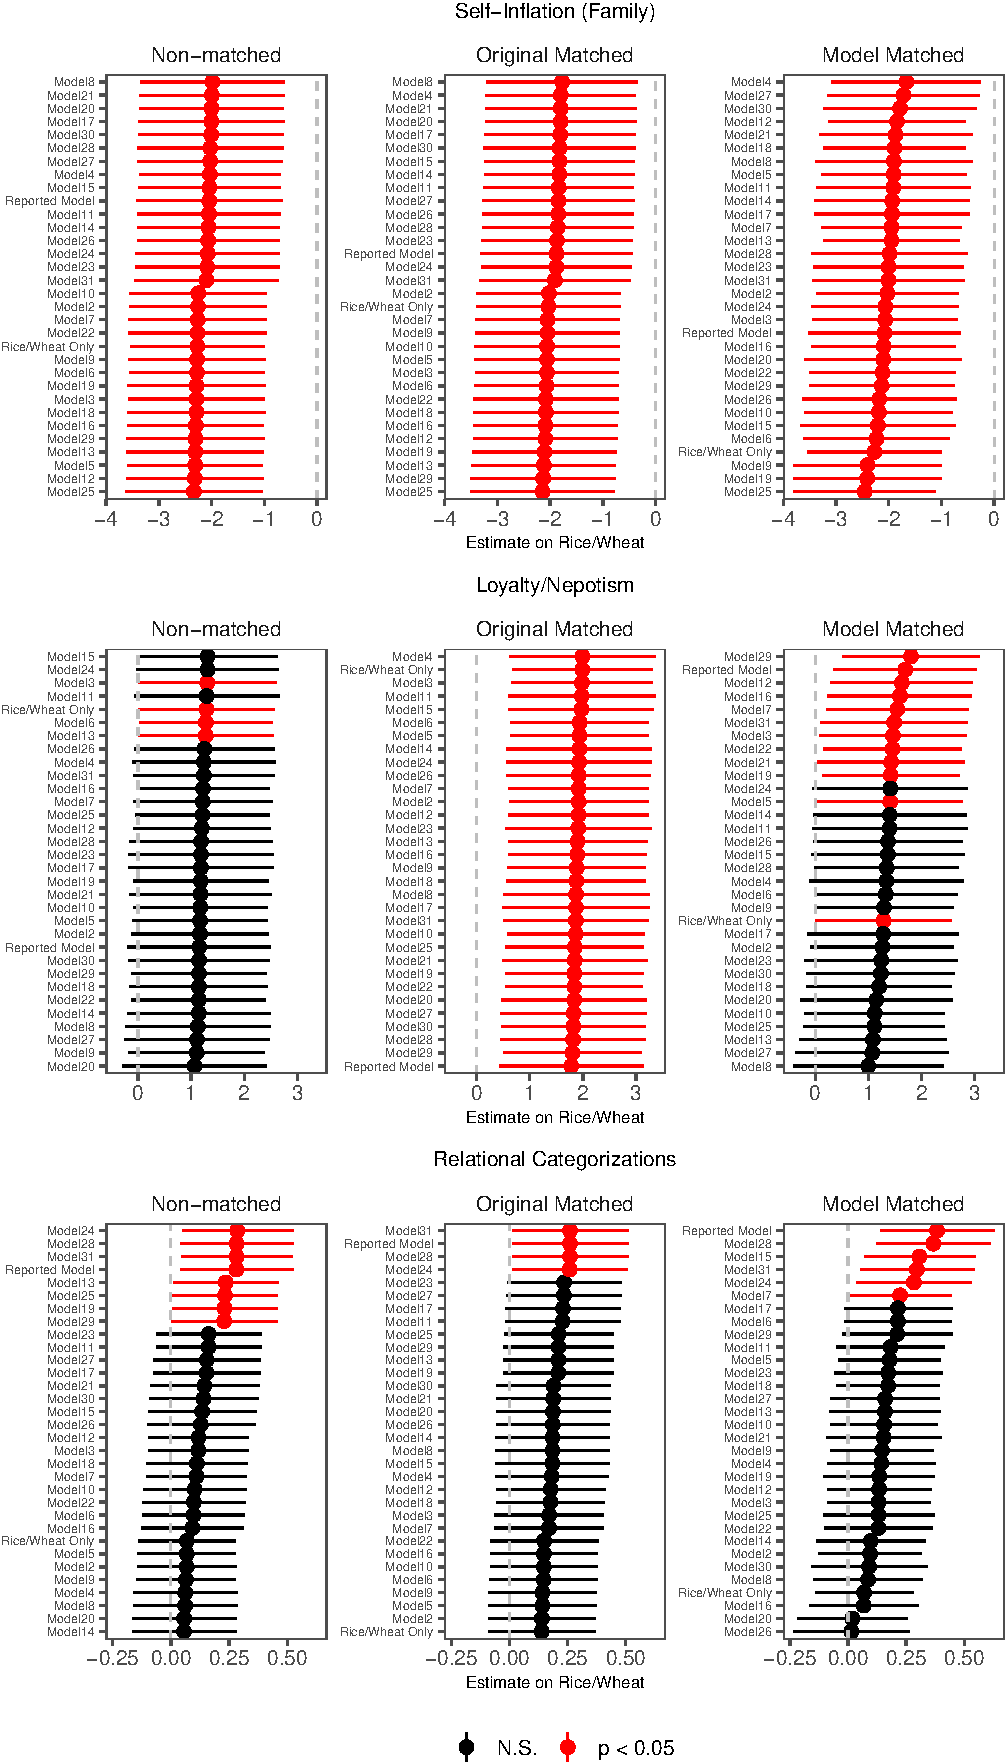
\includegraphics{comment_files/figure-latex/unnamed-chunk-1-1.pdf}
\caption{\label{fig:unnamed-chunk-1} Each panel represents the multiverse analysis for one task. Each point is one estimate on the Rice/Wheat predictor in the particular models. Black dots are the non-significant estimates, and red dots are the significant estimates. 32 models were run for each task. The propensity matching script was retrieved from the OSF repository of Talhelm \& Dong (2024). The script for the reanalysis and the generation of this figure could be found at \url{https://github.com/anjiecao/rice_theory_comment}.}
\end{figure}

In addition to evaluating the results' robustness, it is also critical to examine the key assumptions in this paper: the most important difference between Lianhu and Qukou, two very similar farms, is that one farms rice and the or farms rice. But is this assumption true? As hinted at in the Supplementary Information of Talhelm and Dong (2024), neither Lianhu nor Qukou was a single-purpose farm. According to the farm chronicles, both farms also invested in forestry, fishery and livestock (\emph{Lianhu Farm Chronicles}, 2009; \emph{Qukou Farm Chronicles}, 2010). But more crucially to the test of rice theory is that the ``rice farm'' Lianhu farms wheat, and the ``wheat farm'' Qukou farms rice. Figure 2 shows the historical trend of the proportion of areas within each farm that's dedicated to rice versus wheat. While Lianhu started as a dedicated rice farm, the composition of rice versus wheat rapidly shifted as the farm developed: it became a predominantly wheat farm between 1969 and 1983, and again during the period between 1997-2007. It is worth noting that the majority of the participants in the study were born around 1970, which means that they were born into an era in which wheat is in fact the dominant crop on the farm. Similarly ambiguous patterns can be found in Qukou as well. Although it has stayed as a predominantly wheat and barley farm, the land for farming wheat and barley barely surpasses half of the available land. Moreover, in the 1970s, the rice proportion in Qukou farm was even similar to the rice proportion in the Lianhu farm, hovering around 20\% - 25\%. In other words, this information suggests that the farming practices on the two farms were not as drastically different as depicted.

\begin{figure}
\centering
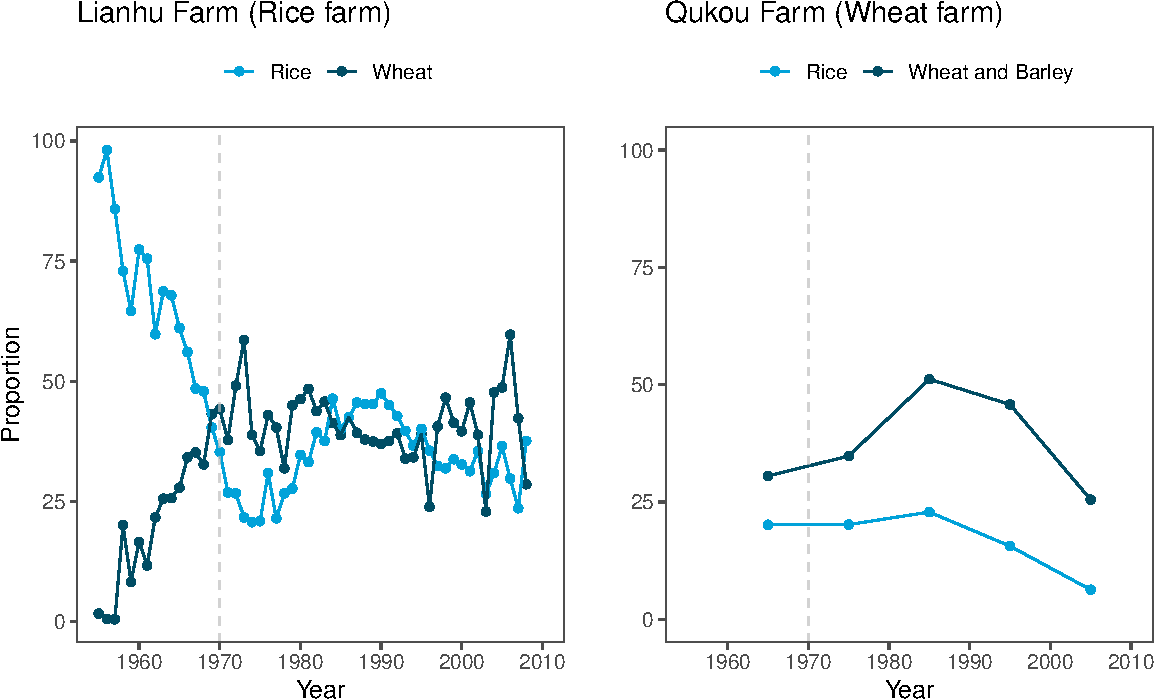
\includegraphics{comment_files/figure-latex/unnamed-chunk-2-1.pdf}
\caption{\label{fig:unnamed-chunk-2}Both pannel show the historical trends of the farm in farming rice versus wheat. Since both farms also farmed other crops, the proportion between rice and wheat (and barley, for Qukou farm) does not add up to 1. The dotted lines represent 1970. 1970 is the year that many participants were born in, which was calculated using the mean age of the participants (47) and the year the study was conducted (2017). Data plotted here was extracted from the two farm chronicles. The raw data can be found in the github repository: \url{https://github.com/anjiecao/rice_theory_comment}.}
\end{figure}

So what else could explain the differences observed in the studies? One hypothesis is the historical background. While both Lianhu and Qukou were state farms, their founding histories could not be more different. Lianhu has a military background. The first residents in Lianhu were military personnel from the First Agricultural Construction Division of the Chinese People's Liberation Army (\emph{Lianhu Farm Chronicles}, 2009). Two years later, veterans from the same division joined. Lianhu Farm experienced tremendous population growth in the first twenty years of their history. Lianhu developed from a tiny farm in 1954 in the middle of a wasteland with only 52 residents to an industrialized farm with 5228 residents in 1974. In contrast, Qukou was never an isolated tiny farm. Qukou's farm chronicle traced the local history back to 114 B.C., suggesting that the area has been inhabited for a long time(\emph{Qukou Farm Chronicles}, 2010). The farm chronicle considers 1960 to be the official founding year of the farm, and by that year, there were already 6256 regular residents. One could imagine that the presence or the absence of the military background could shape how the farms were managed and organized. For instance, the record-keeping differed between the two farms: Lianhu farm has agricultural and population information available in each year, whereas Qukou only has it available every five years. Could the military history and the management style in Lianhu farm cause it to become a more collectivistic farm? Without more information, this question is challenging to answer, but such a significant difference could certainly make it impossible to make direct causal inferences about the farming practices.

This comment is not intended to criticize the rice theory, but to raise questions about whether this particular piece of evidence is suitable for testing the theory. The farming practices between the two state farms were different, but they were not as clear cut as one being the ``rice farm'' and the other the ``wheat farm''. In contrast, the clear contrast in the historical background of the two farms could contribute to the subtle cultural orientation differences observed. I hope this commentary could open the discussion for a more rigorous and more nuanced approach to utilizing historical events as natural experiments for cultural psychology research.

\newpage

\hypertarget{references}{%
\section{References}\label{references}}

\hypertarget{refs}{}
\begin{CSLReferences}{1}{0}
\leavevmode\vadjust pre{\hypertarget{ref-lianhu2009}{}}%
\emph{Lianhu farm chronicles}. (2009). Lianhu Publishing Committee.

\leavevmode\vadjust pre{\hypertarget{ref-qukou2010}{}}%
\emph{Qukou farm chronicles}. (2010). Qukou Publishing Committee.

\leavevmode\vadjust pre{\hypertarget{ref-talhelm2024people}{}}%
Talhelm, T., \& Dong, X. (2024). People quasi-randomly assigned to farm rice are more collectivistic than people assigned to farm wheat. \emph{Nature Communications}, \emph{15}(1), 1782.

\leavevmode\vadjust pre{\hypertarget{ref-talhelm2014large}{}}%
Talhelm, T., Zhang, X., Oishi, S., Shimin, C., Duan, D., Lan, X., \& Kitayama, S. (2014). Large-scale psychological differences within china explained by rice versus wheat agriculture. \emph{Science}, \emph{344}(6184), 603--608.

\end{CSLReferences}


\end{document}
